
% !TEX root = /home/eb/Dropbox/CPGE/Physique/Cours/[4]Optique/[2]Interfer/Figures/fresnel_destruc.tex
\documentclass{article}
\usepackage{tikz}

\begin{document}
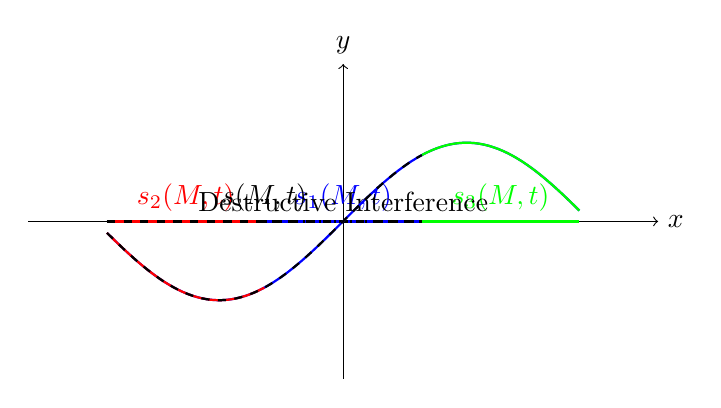
\begin{tikzpicture}
  % Draw the axes
  \draw[->] (-4, 0) -- (4, 0) node[right] {$x$};
  \draw[->] (0, -2) -- (0, 2) node[above] {$y$};

  % Draw the incident wave
  \draw[blue, thick] (-3, 0) -- (3, 0) node[midway, above] {$s_1(M, t)$};

  % Draw the reflected wave
  \draw[red, thick] (-3, 0) -- (-1, 0) node[midway, above] {$s_2(M, t)$};

  % Draw the transmitted wave
  \draw[green, thick] (1, 0) -- (3, 0) node[midway, above] {$s_3(M, t)$};

  % Draw the resultant wave
  \draw[black, thick, dashed] (-3, 0) -- (1, 0) node[midway, above] {$s(M, t)$};

  % Draw the interference pattern
  \draw[black, thick, dotted] (-1, 0) -- (1, 0) node[midway, above] {Destructive Interference};

  % Add phase to all scalar vibrations
  \def\varphi{0.2}
  \draw[blue, thick, domain=-3:3, samples=100] plot (\x, {sin(\x r + \varphi)});
  \draw[red, thick, domain=-3:-1, samples=100] plot (\x, {sin(\x r + \varphi)});
  \draw[green, thick, domain=1:3, samples=100] plot (\x, {sin(\x r + \varphi)});
  \draw[black, thick, dashed, domain=-3:1, samples=100] plot (\x, {sin(\x r + \varphi)});
\end{tikzpicture}
\end{document}
